\documentclass[12pt]{article}
\usepackage[utf8]{inputenc}
\usepackage[margin=3cm]{geometry}
\usepackage{graphicx}
\usepackage{physics}
\usepackage{amsmath}
\usepackage{amssymb}
\usepackage[colorlinks]{hyperref}
\usepackage{subcaption}
\usepackage{babel}
% \captionsetup{font=footnotesize}
\usepackage{booktabs}
\usepackage{multirow}
\usepackage[export]{adjustbox}
\usepackage{floatrow}
\usepackage{listings}
\newcommand{\otoprule}{\midrule[\heavyrulewidth]}
\usepackage{libertine}
\usepackage[T1]{fontenc}
\usepackage[libertine]{newtxmath}
\renewcommand{\d}{\mathrm{d}}
\newcommand{\e}{\mathrm{e}}
\renewcommand{\i}{\mathrm{i}}
\usepackage{pythonhighlight}
\usepackage{amsthm}
\bibliographystyle{plain}
\numberwithin{equation}{section}
\title{A Variational Monte Carlo Method for the Schr\"odinger Equation}
\author{Jack H. Farrell \\ 1003978840}
\date{}
\begin{document}
\maketitle
\tableofcontents
\section{Introduction}
Solving the Schr\"odinger Equation is the center of most quantum mechanical problems, and a number of approaches exist.  However, many methods fail in the areas of atomic, molecular, or solid-state physics --- these complicated situations involve many interacting particles~\cite{sorella_2013}. One popular aproach to handle these many-body systems is the \textit{variational principle}, which involves guessing a form of the wave function and optimizing the exact parameters in order to get the best estimate.  Especially for problems like electrons moving in atoms, molecules, or solids, the variational approach has several advantages over more direct methods for solving partial differential equations.  For one, the method can be efficient --- physical insight can guide a choice of wave functions that have much of the problem ``built in".  As an example, ground state wave functions in one dimension never cross the $x$ axis, and they are often even functions of $x$ ~\cite{shankar_2014}.

The variational principle involves calculating quantum mechanical expectation values, which means in turn computing integrals.  In many-body systems, these integrals can be over large-dimension spaces, since the integration goes over each of the three spatial coordinates associated with each particle.  As such, the Monte-Carlo Method stands out as a promising technique for computing the associated integrals.

This report first introduces the variational principle and outlines how the Monte-Carlo method can be used to facilitate it.  Then, we implement the variational Monte-Carlo and test our code on two classic quantum mechanical ``toy problems".  Finally, we try to extend the method to estimate the ground state energy of the Hydrogen Molecule, $\text{H}_2$.

\section{Methods}
\subsection{The Variational Principle}
Consider a quantum system defined by a hamiltonian $H$, and assume there is a unique ground state $\ket{\psi}$ with energy $E_0$.  In the coordinate basis, we will call the Hamiltonian $\mathcal H$ and the wave function $\psi(\vb*{r})$, where $\vb*r$ has three coordinates.  With these definitions in mind, the variational principle from quantum mechanics says:
\begin{equation}
    \label{eq:variational_principle}
    \frac{\bra\psi H \ket\psi}{\braket{\psi}{\psi}} \geq E_0,
\end{equation}
for any state $\ket\psi$, which does \textit{not} need to be normalized.  In other words, the average energy in any state (the expectation value of the Hamiltonian) must be larger than the ground state energy $E_0$.  The statement can certainly be proved~\cite{shankar_2014}, but it makes sense given that the ground state is defined as the state of lowest energy.

The Variational Principle is a powerful tool for estimating the ground state energy and state vector, $E_0$ and $\ket{\psi_0}$, of a quantum system that can not be solved exactly. To do so, we first decide on a \textit{trial wave function} that has some particular form and depends on some parameter(s).  For example, in one dimension with one paramter, we could have $\psi_\alpha(x) = \e ^{-\alpha x}$. In that case, we would be picking a trial wave function of the form of an exponential and treating the decay width as a parameter $\alpha$. Then, according to Eq.~(\ref{eq:variational_principle}), and defining $E[\ket\psi] \equiv \bra\psi H \ket\psi / \braket{\psi}{\psi}$, we have:
\begin{equation}
    E[\ket{\psi_\alpha}] \equiv \frac{\bra{\psi_\alpha} H \ket{\psi_\alpha}}{\braket{\psi_\alpha}{\psi_\alpha}} \geq E_0.
\end{equation}
The value here will be different for each value of $\alpha$.  To get the best estimate of the ground state, then, which will be the closest upper bound to $E_0$, we need to minimize $E[\psi_\alpha]$ with respect to the parameter $\alpha$.  In the case of the exponential trial wave function, we will then be able to find the ``best estimate of the ground state for all wave functions that are exponentials.

Of course, the accuracy of the estimate depends strongly on how sensible the form of the trial wave function was.  That means, when we get to solving problems, we should work to create physically reasonable trial wave functions.

\subsection{Variational Monte Carlo}
The explanations here come, roughly, from~\cite{jensen}, \cite{Jensen2}, and ~\cite{sorella_2013}.  In some simple cases, the minimization described in the last section can be performed analytically: once one computes the matrix elements and has an estimate for the energy $E(\alpha)$ as a function of $\alpha$, all that is left os to compute the derivative $\dv{E(\alpha)}{\alpha}$ and set it equal to $0$, a normal minimization problem.  In other situations, though, especially in many-particle situations when the matrix elements depend on integrals over spaces of large dimension, just computing this integral can be a challenge.  As we saw in class, the Monte-Carlo Method can solve high-dimensional integrals.

Since we will be working in the coordinate representation, let us define $\vb*r$ to .In quantum mechanics, the probability distribution assocated with a wave function is:
\begin{equation}
    \rho(\vb*r) \equiv \frac{\left| \psi_\alpha(\vb*r) \right|^2}{ \int\d \vb*r \left| \psi_\alpha(\vb*r) \right|^2}.
\end{equation}
Here, by $\d \vb*r$, we mean the volume element in whatever dimension we are working. Additionally, one can define the so-called \textit{local energy operator}:
\begin{equation}
    E_L(\alpha) = \frac{\mathcal{H}\psi_\alpha(\vb*r)}{\psi_\alpha(\vb*r)}
\end{equation}
The purpose of these definitions is to be able to write the variational principle in a suggstive way --- rewriting Eq.~(\ref{eq:variational_principle}) using the new definitions, we obtain:
\begin{align}
    \label{eq:statistical}
    E \left[ \psi_\alpha(\vb*r) \right] = \int \d \vb*r \rho_\alpha(\vb*r) E_L(\vb*r).
\end{align}
This equation says that computing the \textit{quantum-mechanical} expectation value of $H$ is the same as computing the \textit{statistical} weighted average of the local energy $E_L(\vb*r)$ according to the probability distribution $\rho$~\cite{newman_2013}.

\subsection{Metropolis Algorithm}
Using Monte-Carlo integration to compute the integral in Eq.~(\ref{eq:statistical}) requires random numbers drawn from the distribution $\rho$, but, like the thermodynamics case, sampling from such a generally complicated distribution can be challenging.  Instead (also like the thermodynamics case), we can generate positions with the appropriate probabilities using the Markov Chain Method and the Metropolis Algorithm.

Say we start a virtual electron (called a "random walker" in the literature) at the position $\vb*r$, and we compute a random step $\Delta \vb*r$.  We need to compute the ratio:
\begin{equation}
    \mathcal{R} = \frac{\rho_\alpha(\vb*r + \Delta \vb*r)}{\rho_\alpha(\vb*r)}.
\end{equation}
Then, we decide whether or not to ``accept" the step according to the following algorithm:
\begin{enumerate}
    \item If $\mathcal{R} > 1$, then accept the step,
    \item If $\mathcal{R} < 1$, then accept the state with a probability $\mathcal{R}$.
\end{enumerate}

\section{Results}
Before moving on to more complicated systems, we use the variational method to solve some exactly solvable problems.  Comparison the the exact ground state energy will motivate some methods of determining the error in our approach.  We note that we follow closely the setup of ~\cite{jensen}.
\subsection{Simple Harmonic Oscillator}
First, consider a particle moving in one dimension, whose wave function $\psi$ obeys the Sch\"{o}dinger equation:
\begin{equation}
    \mathcal H = -\frac{\hbar^2}{2m} \pdv[2]{x}\psi(x) + \frac12m \omega^2 x^2 = E\psi(x).
\end{equation}
If we work in units where $E \rightarrow E / \hbar \omega$, $x \rightarrow \sqrt{m\omega / \hbar} x$, we achieve the simpler:
\begin{equation}
    \mathcal H = -\frac{1}{2} \pdv[2]{x}\psi(x) + \frac12 x^2 = E\psi(x).
\end{equation}
As a trial wave function, we consider:
\[ \psi_\alpha(x) = \e ^{-\alpha^2 x^2 / 2} = E \psi(x),\]
in other words, a Gaussian function.  Note that $\alpha$ should be measured in units of $\hbar/m\omega$, the opposite of the units of $x$. Since this function agrees with the exact ground state when $\alpha = 1$, our calculations should find a minumum in the energy $E\left( \alpha \right)$ at $\alpha = 1$.  Further, the energy should be $E(\alpha = 1) = 1/2$, the ground state energy of the simple harmonic oscillator in this case.

We ran the code at 50 equally spaced values of $\alpha$ in the interval $(0, 2)$.  At each value of $\alpha$, we performed $N = 100 000$ Metrolpolis Steps.  After $N$ steps, we computed the mean of $E_L$ and the standard deviation $\sigma$.

Fig.~(\ref{fig:sho}) shows the average of $E_L(x)$, which is also the quantum mechanical expectation value $E(\alpha)$ as a function of the variational parameters $\alpha$.
\begin{figure}[ht]
    \centering
    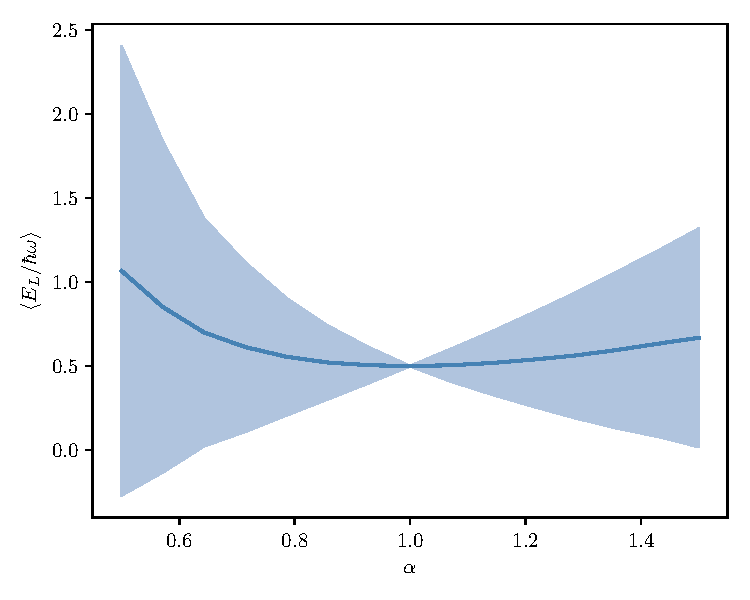
\includegraphics{../scripts/sho.pdf}
    \caption{Simple harmonic oscillator in dimensionless units.  We used $N = 100 000$ steps and a maximum markov chain step of 2.  The trace givse the average value of the local energy as a function of the variational parameter $\alpha$, and the lighter envelope gives the standard deviation, which approaches 0 near the exact solution.}
    \label{fig:sho}
\end{figure}
Two features stand out from the figure.  First, the solid trace in the figure shows a clear minimum at $\alpha \approx 1$, with a minimum value $E(1) \approx 0.5$.  This result agrees with the exact solution, as it should.  Secondly, the lighter ``envelope", which gives the standard deviation $\sigma$ of the average $\langle E_L(x) \rangle$, becomes small in the exact solution.  As we expect, the exact solution has zero variance.  Running more steps monte carlo steps would further decrease the variance, and the method would return a closer to the exact solution.  With our simulation involving $N = 100 000$ steps, we achieve a result (the minimum energy):
\begin{equation}
    E_0 = (0.5000 \pm 0.0004) \hbar \omega. \nonumber
\end{equation}
The result is in excellent agreement with the exact solution of $\hbar \omega / 2$

\subsection{Hydrogen Atom}
Now, imagine a particle moving in three dimensions near a hydrogen nucleus.  The wave function $\psi(\vb* r)$ obeys the Sch\"odinger equation:
\begin{equation}
    \frac{\hbar^2}{2\mu}\grad^2\psi(\vb*r) - \frac{e^2}{r}\psi(\vb*r) = E \psi(\vb*r).
\end{equation}
Here, $r = |\vb* r|$, $\mu = \frac{m_e m_p}{m_e + m_p}$ is the ``reduced mass" of an electron-proton system, $\grad^2 = \pdv[2]{x} + \pdv[2]{y} + \pdv[2]{z}$ is the Laplacian operator, and $e$ is the charge of the electron in CGS units.  Again, it is useful to instead work in units where: $E \rightarrow E \hbar^2 /\mu e^4$, $\vb*r \rightarrow \vb*r / a$ where $a = \hbar^2 / me^2$.  That corresponds to measuring the electric charge in units of $e$, i.e., $e=1$ in these units.  We get a simplified equation:
\begin{equation}
    \frac12\grad^2\psi(\vb*r) - \frac{1}{r}\psi(\vb*r) = E \psi(\vb*r).
\end{equation}

Again, we ran the simulation, this time with $N=50 000$ Monte-Carlo steps.  Fig.~(\ref{fig:hydrogen_atom}) shows the result .
\begin{figure}[ht]
    \centering
    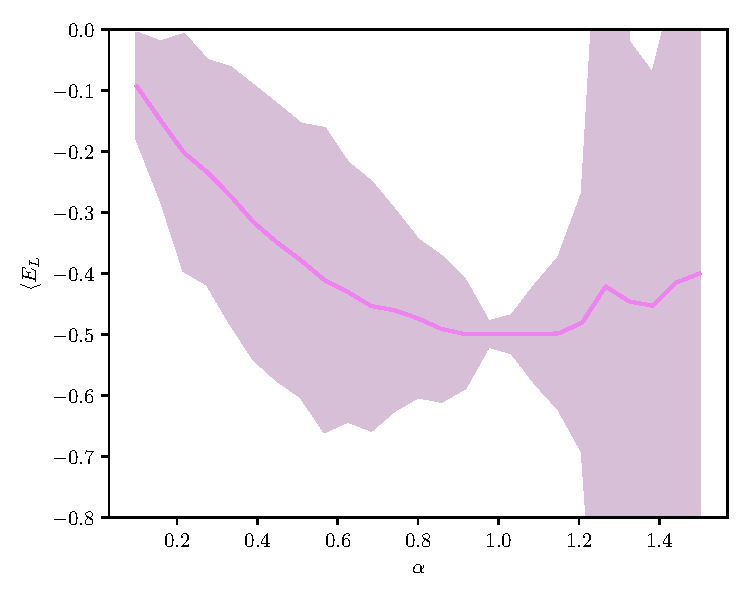
\includegraphics{../scripts/hydrogen_atom.pdf}
    \caption{Hydrogen atom in dimensionless units.  We used $N = 50 000$ steps and a maximum markov chain step of 2.  The trace givse the average value of the local energy as a function of the variational parameter $\alpha$, and the lighter envelope gives the standard deviation, which approaches 0 near the exact solution.}
    \label{fig:hydrogen_atom}
\end{figure}
In these units, the exact solution should be $E_0 = -0.5$. (T)


\subsection{The Hydrogen Molecule}
\subsubsection{Setup}
Now, having established the method, we will \textit{try} a harder problem, the Hydrogen molecule.  The idea for this part of the setup comes from a problem listed in \cite{Jensen2}.Now, we   In this case, we have two electrons moving near two force centers.  The positions of the electrons are $\vb*{r_1}$ and $\vb*{r_2}$, and the positions of the atoms are $\vb*{R_1}$ and $\vb*{R_2}$.  They each feel a force from each proton, and there is also an interaction between the electrons.  The Hamiltonian, in the coordinate basis, is:
\begin{equation}
    -\frac12 \grad_1^2 - \frac12 \grad_2^2 - \frac{1}{|\vb*r_1 - \vb*R_1|}- \frac{1}{|\vb*r_1 - \vb*R_2|}- \frac{1}{|\vb*r_2 - \vb*R_1|}- \frac{1}{|\vb*r_2 - \vb*R_2|} + \frac{1}{|\vb*r_1 - \vb*r_2|}
\end{equation}

To apply the variational method, we will choose an ansatz wave function that is a linear combination of atomic orbitals (LCAO). That means we take each particle's wave function to have the form:
\begin{equation}
    \phi(\vb*r) = \frac{1}{\sqrt{2}}\left( \phi_{\text{1s}}(\vb*r - \vb*R_1) +  \phi_{\text{1s}}(\vb*r - \vb*R_2) \right).
\end{equation}
Here, by $\phi_{\text{1s}}$ we mean the ground state wave functions for a one-electron atom of charge $Qe$ where $e$ is the charge of the electron.  In other words, it is a linear combination of the atomic wavefunctions centered at each of the two atoms in the Hydrogen molecule.  Since the force from each atom has the same strength, it makes sense that the two wavefunctions get equal weight in the linear combination; there is no atom to which the electrons ``prefer" to be close.

Further, instead of just $Q = 1$, the case for the Hydrogen atom, we can note that, physically, the repulsion from the other electron will effectively screen the interaction.  To model this effect, we will treat the effective $Q$ that appears in the 1S orbitals as a variational parameter --- we expect to find $Q < 1$ will be favoured.  That means atomic ground state looks like:
\begin{equation}
    \phi_{\text{1s}}(\vb*r_1) \propto \e ^{-Q r}
\end{equation}

We will also use a second variational parameter --- the distance between the two atoms that make up the Hydrogen molecule, which we will call $d$.  We take the two atoms to be at positions $\vb*R_{1,2} = \pm \frac{d}{2}\vu*z$.

\subsubsection{Results}
A wide range of minimization algorithms exist for finding the minima of functions that depend on more than one parameter.  Here, we use the simple approach of making a grid of $d$ and $\alpha$ values that we will use, and tabulating the calculated energy at each pair.  Then, we simply take the minimum over that range.  This is a computationally intensive procedure that limited our accuracy given the time scale of the project.  We used a 50$\times$50 grid of values of $\alpha$ and $d$, and ran the simulation at only 500 MC steps for each of the 2500 grid points.  The low number of steps is a major source of error.

With this choice, we found an optimal value of  $d$ that was:
\begin{equation}
    d = 1.396.
\end{equation}
This is quite close to the true value of around $1.400$ in units of the Bohr Radius, which we had called $a$ earlier in this report \cite{Jensen2}.  However, at this value of $d$, Fig.~(\ref{fig:molecule}) gives the average energy.
\begin{figure}[ht]
    \centering
    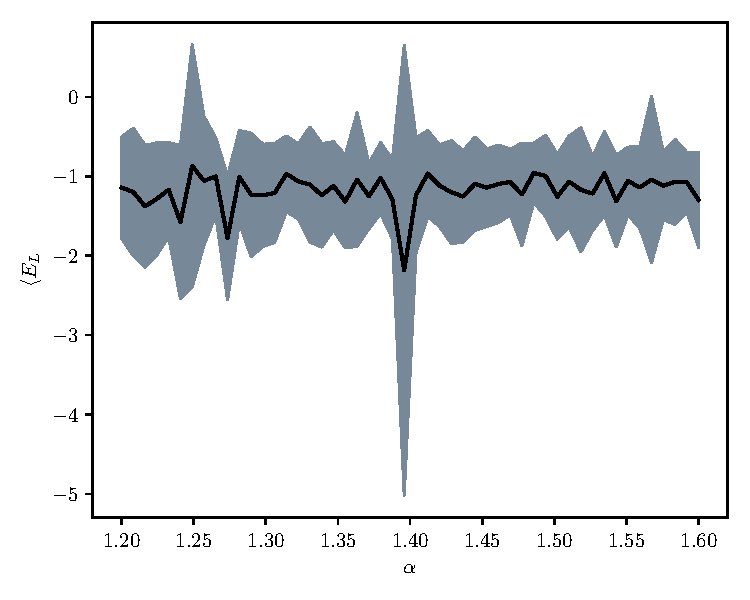
\includegraphics{../scripts/hydrogen_molecule1.pdf}
    \caption{Hydrogen molecule in dimensionless units. We have fixed $d = 1.396$ and plotted the average energy as a function of $\alpha$. We used $N = 500$ steps and a maximum markov chain step of 2.  The trace givse the average value of the local energy as a function of the variational parameter $\alpha$, and the lighter envelope gives the standard deviation, which approaches 0 near the exact solution.}
    \label{fig:molecule}
\end{figure}
The error bars are substantial, leading to a quite imprecise result for the average ground state energy:
\begin{equation}
    E = -2.1 \pm 2.
\end{equation}
Running the simulation for more steps may have yielded better results.  This less-than-stellar outcome motivates a discussion of optimizations and errors for a stronger method.

\section{Discussion}
Our implementation gave excellent results for the two toy problems and good results for the Hydrogen Atom.  Still, aspects of the code could be improved, especially in two key areas.

\subsection{Optimization}
In the code, we already made some important optimizations.  The most important is that computing the local energy as we defined it does \textit{not} require computing the norm of the state, which would be computationally challenging, especially in large problems with more electrons.

For systems of more electrons, we would need to implement the following idea to make the method reasonable.  One step in the Metropolis algorithm requires computing a ratio of the probability densities, $\rho_\alpha$ --- but, in general, changing the state of one particle will not effect the rest of the system.  In that way, there is no need to compute the rest of the system again:

\subsection{Evaluation of Errors}
The method we have presented has several sources of error.  First of all, physically.

Quantitatively, a simple and robust method to quantify the error is to examine the standard deviation of the local energy $E_L$ that we were computing in each case.  This is a good option for quantitatively understanding the error of the method because it takes both the physical and computational errors into account.  Physically, we expect that an exact eigenstate of the Hamiltonian will have zero quantum-mechanical uncertainty in the result, reflecting that we expect low variance when we compute the statistical average of $E_L$.  Secondly, computing the standard deviation reflects errors in our method since the technique involved random numbers and statistics.

When we solved the the first two problem, harmonic oscillator and hydrogen atom, using, in each case, an ansatz that was also the exact solution, we obtained negligible standard deviations.  However, when we solved the Hydrogen molecule, our result yielded substantial standard deviation.  Our hypothesis is that the error depends strongly on the amount of samples: as we expected, 500 steps in the Monte Carlo method was too little to get statistically significant result.

Additionally, in calculating the optimal values of the $\alpha$ parameters, we must note that we only used a finite grid of possibilities, so we must use the grid spacing as an error as well.

\section{Conclusion}
The problem of the Hydrogen Molecule proved challenging and computationally intensive.  Stil, the variational monte carlo method proved useful in terms of obtaining an estimate.  Further, in a one dimensional and a three dimensional test case, the method gave excellent results with little error compared to the exact solutions.

Future projects could investigate the wide array of extensions, optimizations, and refinements of the variational monte carlo method, as well as more complicated methods like Diffusive Monte Carlo or Density Functional Theory methods.  Another avenue is to continue using a variational approach, but to develop a more complicated ansatz that better approximates the physics of the situation.  Overall, the physical insight required to generate an ansatz and the robustness of monte carlo integration make the variational monte carlo an elegant and useful method for solving atomic problems.

\bibliography{bibliography}{}

\end{document}
